\section{Synchronous drive}

A synchronous drive robot is a sophisticated mechanical robot design incorporates three wheels for both propulsion and steering.
It employs two motors: one for driving the wheels and another for steering them. 
All wheels are oriented in the same direction to ensure smooth movement.
Additionally, the robot may include an extra actuator for precise control of angular velocity $\omega$.
\begin{figure}[H]
    \centering
    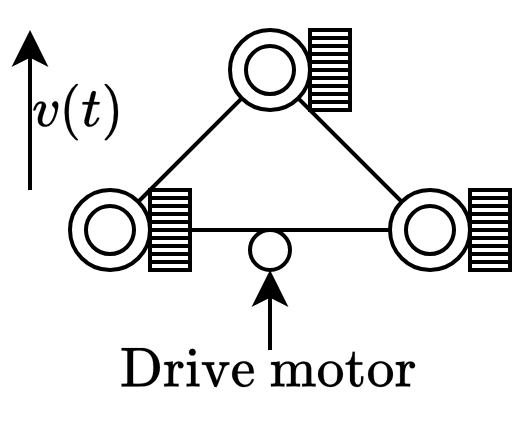
\includegraphics[width=0.25\linewidth]{images/syn.png} 
    \caption{Synchronous drive robot}
\end{figure}
The robot's control variables consist of the linear velocity $v(t)$ and the angular velocity $\omega(t)$. 

Its Instantaneous Center of Curvature remains at infinity, indicating non-holonomic behavior where the robot can only translate freely.

For the synchronous drive of the robot:
\begin{itemize}
    \item Both linear velocity $v(t)$ and angular velocity $\omega(t)$ are directly controlled.
    \item Steering adjusts the direction of the Instantaneous Center of Curvature (ICC).
\end{itemize}
\begin{figure}[H]
    \centering
    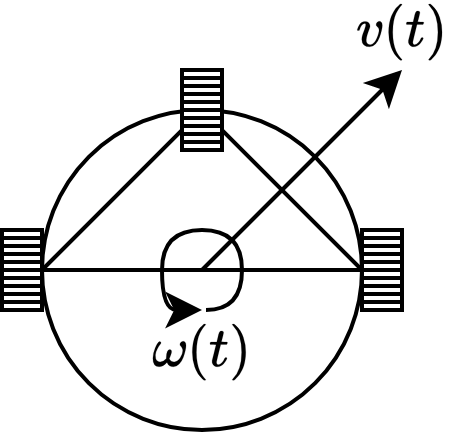
\includegraphics[width=0.25\linewidth]{images/syn1.png} 
\end{figure}
In this configuration, when $v(t)=0$ and $\omega(t)=\omega$ at a specific time instant, the robot rotates in place. 
Conversely, when $v(t)=v$ and $\omega(t)=0$ at a particular time instant, the robot moves linearly. 

\subsection{Odometry}
To compute the velocity in the base frame, we use the following equations:
\[\begin{cases}
    v_x = v(t) \cos (\omega(t)) \\
    v_y = v(t) \sin (\omega(t))
\end{cases}\]
Integrating the position in the base frame, we obtain the robot odometry:
\[\begin{cases}
    x(t)=\int_0^t \cos\left(\theta(t^\prime)\right) dt^\prime \\
    y(t)=\int_0^t \sin\left(\theta(t^\prime)\right) dt^\prime \\
    \theta(t) = \int_0^t\omega(t^\prime) dt^\prime
\end{cases}\]